



\section{Synthetic Experiments}
\label{sec:syn_exp}
In this section, we evaluate our two tests and the resulting lower bounds in finite-sample synthetic and semi-synthetic experiments. In particular, we fix the true unobserved confounding strength $\Gammatrue$ and conduct experiments varying the sample size and the invariant distribution $\pinv$. 

First, we postulate that, for a fixed $\Gammatrue$,
the tightness of 
the lower bound $\gammalb$ improves when the confounder $U$ is more informative about the potential outcomes $(Y(1),Y(0))$. In our experiments, we choose the correlation between 
the unobserved confounder and one of the potential outcomes as a proxy measure of information,
\begin{equation}  
\label{eq:correlation}
\rho_{u,y} = \frac{\operatorname{Cov}_{\pfullobs}[Y(1),U]}{\sigma_{Y(1)} \sigma_U}.
\end{equation}
Intuitively, the sensitivity analysis bounds are tight for a specific $\Gammatrue$ when $\pcnfos$ leads to a marginal distribution $\pobs$ that maximally biases the estimable ATE. This situation occurs, for instance, when patients experiencing smaller outcomes are assigned to the control group while those with larger outcomes are in the treatment group. In this case, the sensitivity analysis bounds must be sufficiently large to include the true ATE and remain valid. 
Such a scenario is only possible if $U$ is very informative of $Y(1)$, captured by a high correlation coefficient. 
Conversely, when the confounder carries little information about the potential outcomes, the sensitivity bounds are unnecessarily conservative, leading to low power of the test and hence looser $\gammalb$. More formally, \Cref{apx:limitations_msm} discusses two extreme cases. If the unobserved confounder is maximally informative about the potential outcomes, namely \(U=(Y(1),Y(0))\), then \(\gammalb\) converges to \(\Gammatrue\) in the infinite-sample limit. Conversely, if \(U \indep (Y(1),Y(0))\), then the confounder carries no information about the potential outcomes and \(\gammalb \) converges to $1$. 
 

Second,  we study the behavior of the lower bound as the observational study sample size grows. In real-world situations, increasing the number of samples in a randomized trial is often constrained by the logistical challenges of conducting additional experiments. However, observational studies have the potential for continuous growth through electronic health records and insurance claims databases. In the context of postmarketing, ongoing monitoring enables the inclusion of data from newly exposed individuals. Therefore, we compare our two tests when the sample size of the observational study grows: our experiments show that $\test_{\obsres}$ has better statistical power when $\nobs$ is large.
\subsection{Datasets}
\label{sec:datasets}
\paragraph{Synthetic distribution} We first benchmark tests and respective lower bounds with a synthetic distribution similar to \citep{yadlowsky2022bounds,jin2023sensitivity}. Here, the propensity score, the true unobserved confounding strength $\Gammatrue$, and the correlation strength can be designed.


We choose the invariant $\pinv$ to be the following linear outcome model 
$$
Y(T)= (2 T-1) X+(2 T-1) + U +\epsilon, \quad \epsilon \sim \gauss(0,\sigma^2_Y).
$$
For the marginal distribution over $X,U$ in $\pconf^{\diamond}$ we generate an unobserved confounder $U \sim \operatorname{Unif}(0,1)$ for both study designs and draw the observed covariate according to
$$ \prct_X = \operatorname{Unif}(-1,1), \; \pobs_X =  \operatorname{Unif}(-2,2).$$
Further, for the observational distribution, we choose the conditional distribution of the treatment $T$ given $X,U$ to be a  Bernoulli, which satisfies the marginal sensitivity model with an odds ratio equal to $\Gammatrue$.
Specifically, we fix the marginal propensity score as $$\pconfobs(T=1 \mid X)=\logit\left(0.75X + 0.5\right),$$ and design the full propensity score  $\pconfobs(T=1 \mid X, U)$ such that it marginalizes to $\pconfobs(T=1 \mid X)$.
For the randomized control trial, we choose 
$\pi = \pconfrct (T=1| X,U) = 1/2$.
We refer the reader to~\Cref{apx:syn_exp} for complete experimental details. 






\paragraph{Semi-synthetic datasets} We expand our benchmark using three real-world randomized trials: Hillstrom's MineThatData Email data~\citep{hillstrom2008}, the Tennessee STAR study~\citep{word1990state} and the VOTE dataset~\citep{gerber2008social}.
In contrast to the synthetic experiments, these datasets involve real outcome functions, though the treatment assignment is still controlled. 

We focus on Hillstrom's dataset for clarity of presentation, and we refer the reader to~\Cref{apx:additional_experiments} for experiments on the other datasets showing similar trends. \citet{hillstrom2008} focused on measuring the impact of an email campaign on the dollars spent by the recipients in the following two weeks. We first sample a small subset of the original trial, $D$, as our randomized trial, $\datarct$. We can then subsample multiple observational studies from $D \setminus \datarct$ sharing a fixed true confounding strength $\Gammatrue$, i.e. $\pconf$, but with a varying correlation between the hidden confounder $U$ and outcome $Y(1)$, i.e. $\pinv$. 

Let us denote $\Xall$ as the vector of all observed covariates. While we cannot intervene on $\pinv (Y(1), Y(0)|\Xall)$ as it is intrinsic to the dataset, we can generate multiple observational studies by partitioning $\Xall$ into unobserved $U$ and observed $X$ in different ways.
For a given partitioning $\Xall = (U,X)$, the resulting $\dataobs$ will have a specific  $\pinv (Y(1), Y(0)|U)$  and hence correlation coefficient $\rho_{u,y}$. With each choice of $U$, we enforce a propensity score $\pconfobs(T=1 \mid U)$ that satisfies $\msm(\pobs, \Gammatrue)$
by subsampling $D \setminus \datarct$. Finally, we remove $U$ to construct $\dataobs$. Our subsampling approach is a variation of the methods presented in~\citet{keith2023rct, gentzel2021and} (see further details in Appendix \ref{apx:semisyn_exp}). Finally, we enforce \Cref{asm:nested_support} by excluding urban zip codes from the support of the randomized trial.

\begin{figure*}
\vspace{-9mm}
    \centering
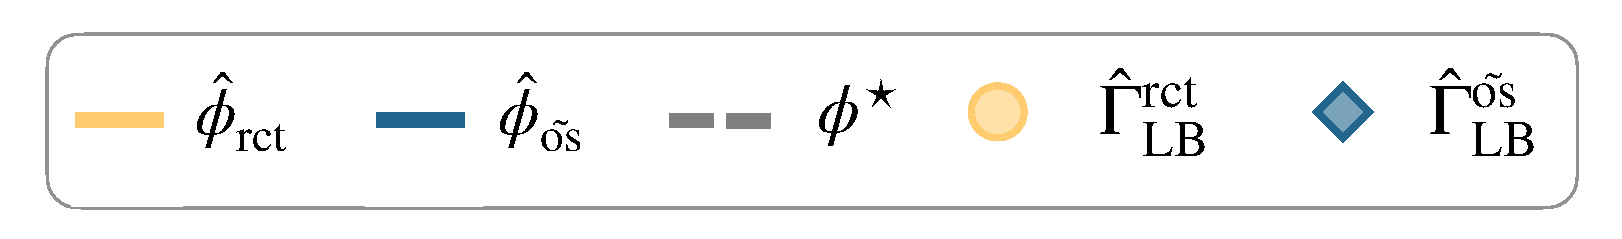
\includegraphics[scale=0.25]{legend}
      \\
    \begin{subfigure}[b]{0.24\textwidth}
        \centering
      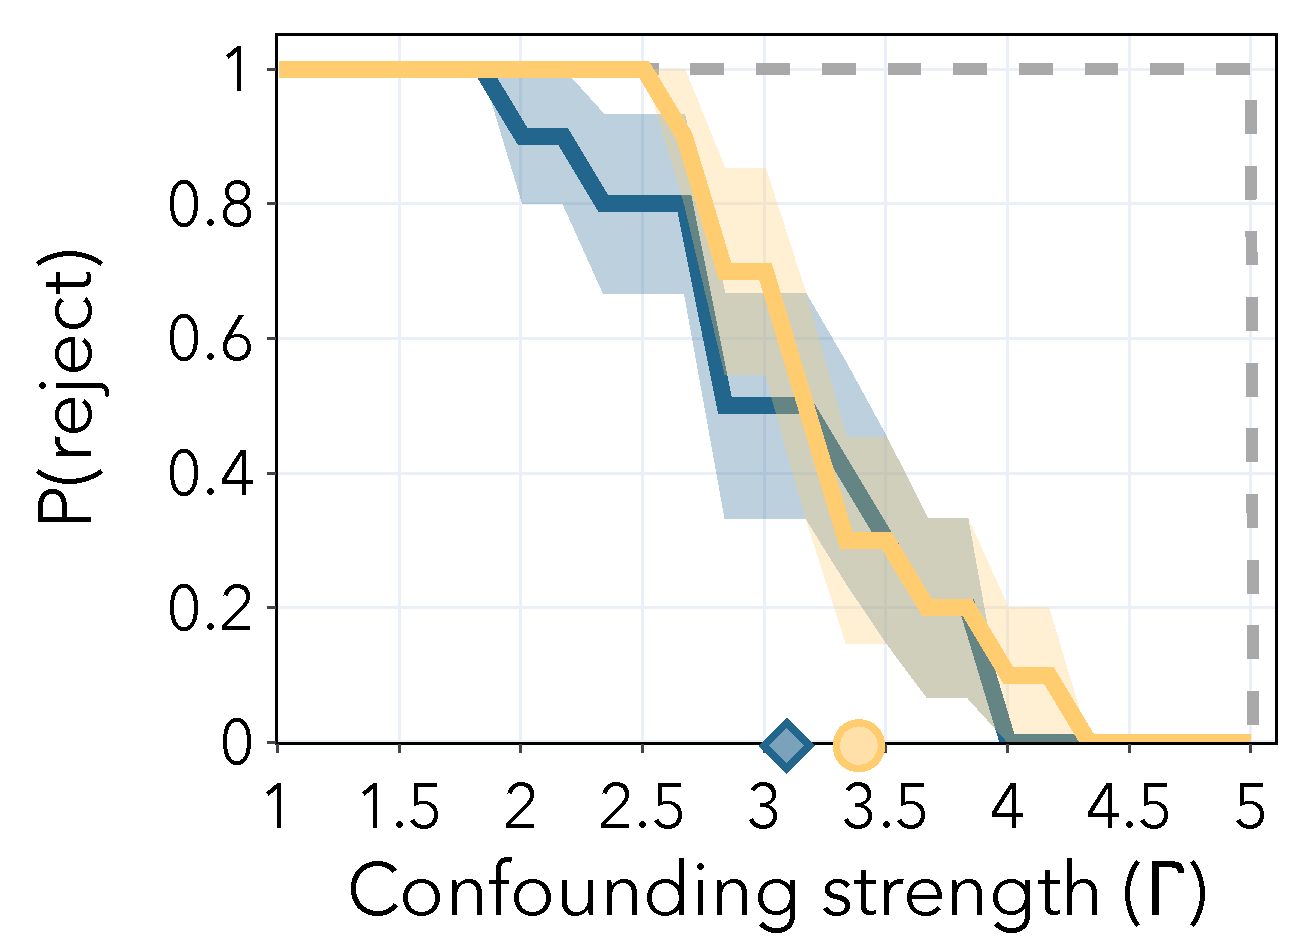
\includegraphics[width=\textwidth]{synthetic_small}
        \caption{\footnotesize{Small sample (synthetic)}}
   \label{fig:synthetic_small_sample}
    \end{subfigure}
    \hfill
    \begin{subfigure}[b]{0.24\textwidth}
        \centering
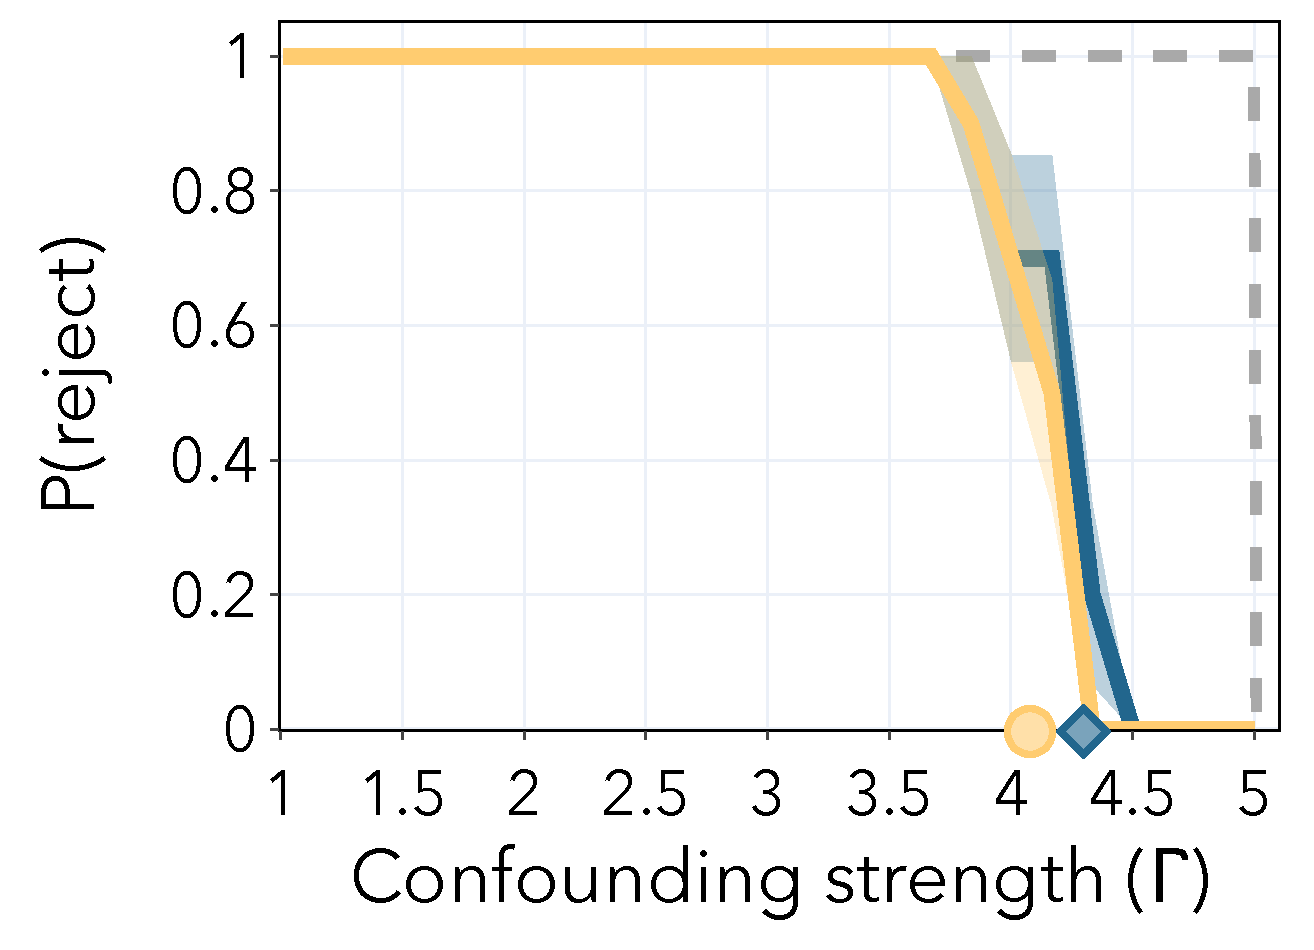
\includegraphics[width=\textwidth]{synthetic_large}
        \caption{\footnotesize{Large sample (synthetic)}}
    \label{fig:synthetic_large_sample}
    \end{subfigure}
    \hfill
    \begin{subfigure}[b]{0.24\textwidth}
        \centering
   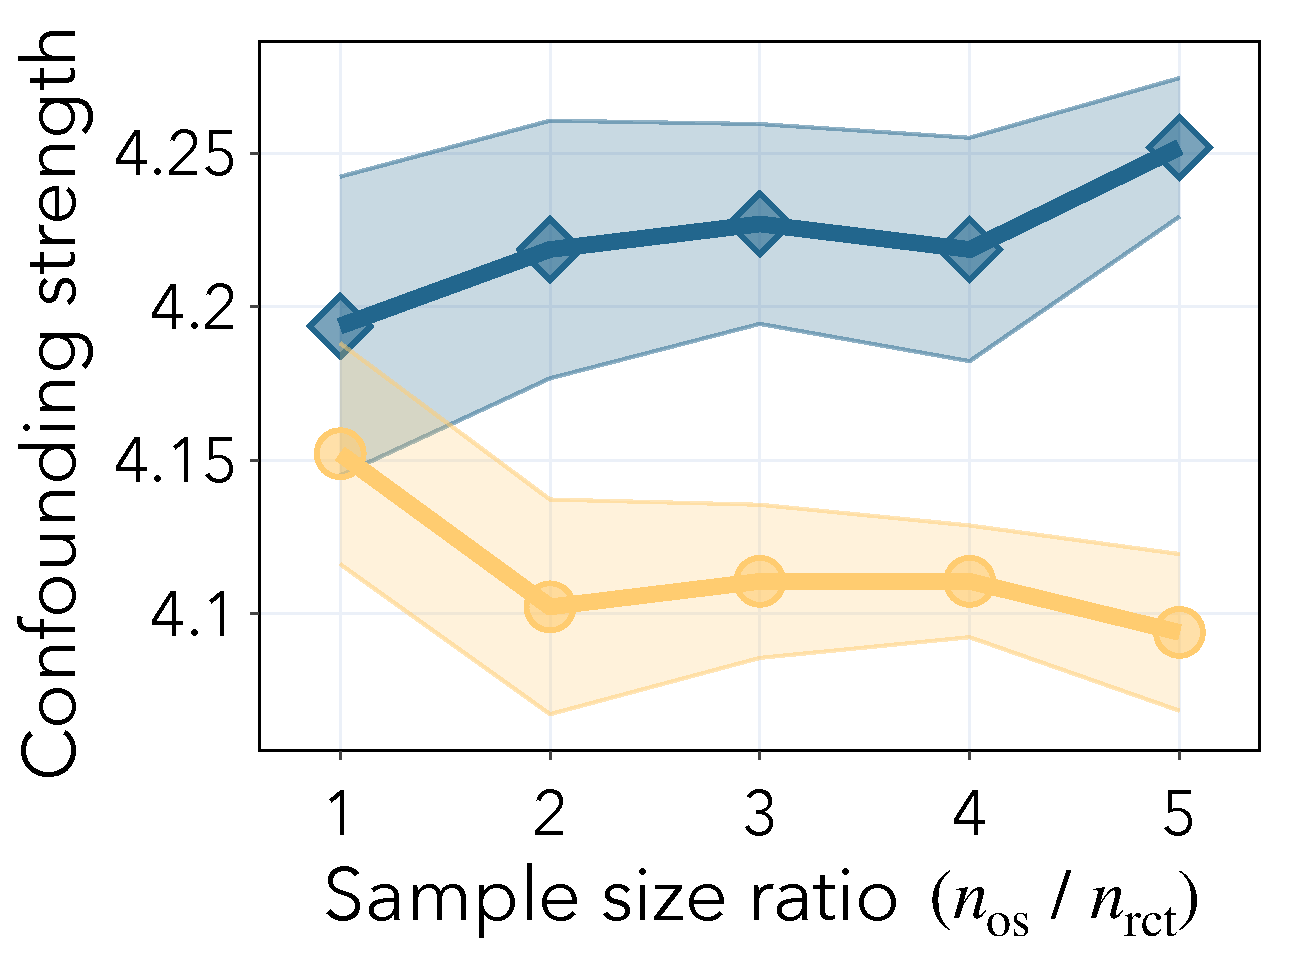
\includegraphics[width=\textwidth]{synthetic_nobs}
        \caption{\footnotesize{Increasing $\nobs$ (synthetic)}}
        \label{fig:synthetic_obs_sample}
    \end{subfigure}
    \hfill
    \begin{subfigure}[b]{0.24\textwidth}
        \centering
    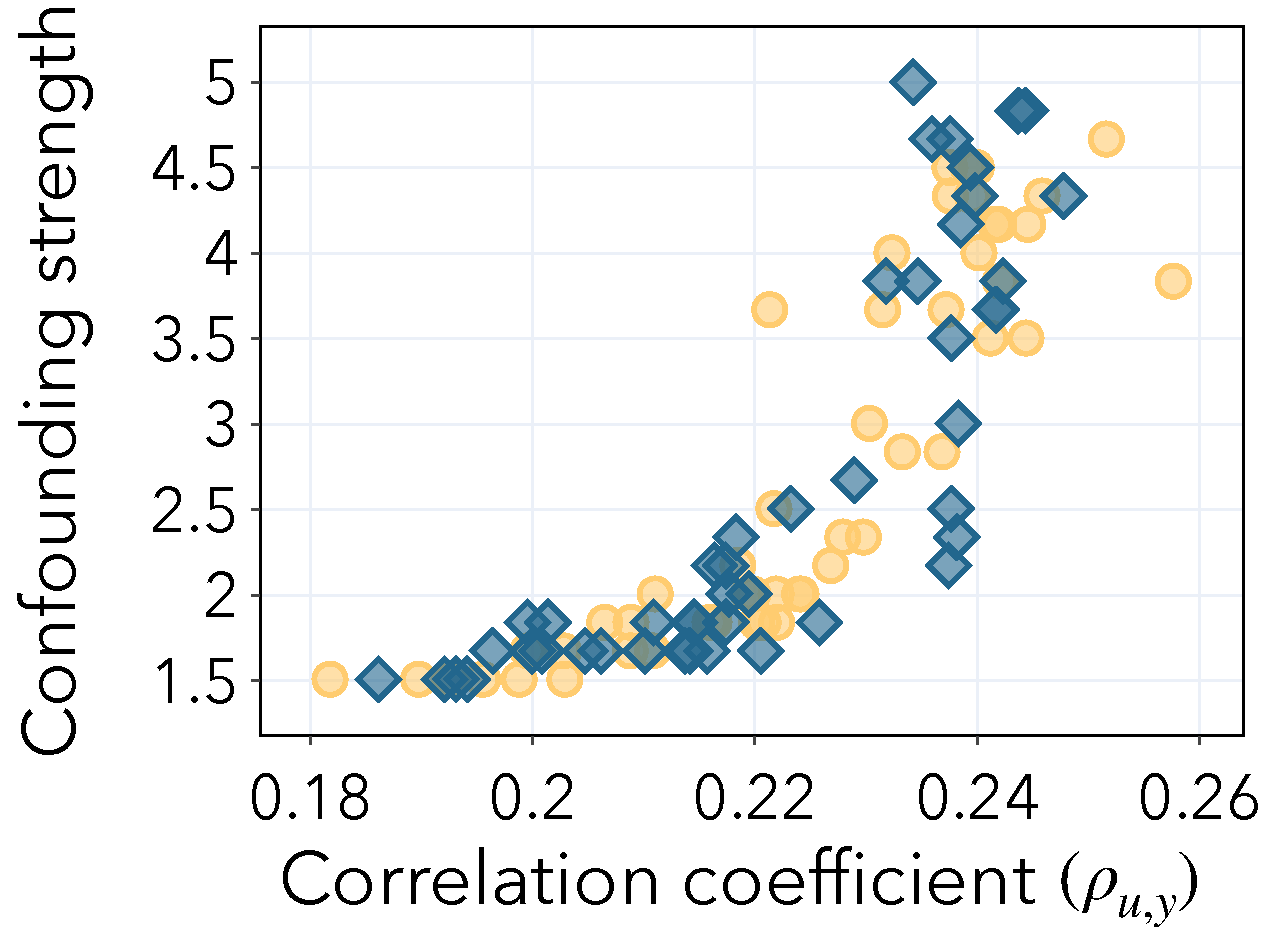
\includegraphics[width=\textwidth]{synthetic_correlation}
        \caption{\footnotesize{$\rho_{u,y}$ effect (synthetic)} }
     \label{fig:synthetic_correlation}

    \end{subfigure}\\
    \begin{subfigure}[b]{0.24\textwidth}
        \centering
    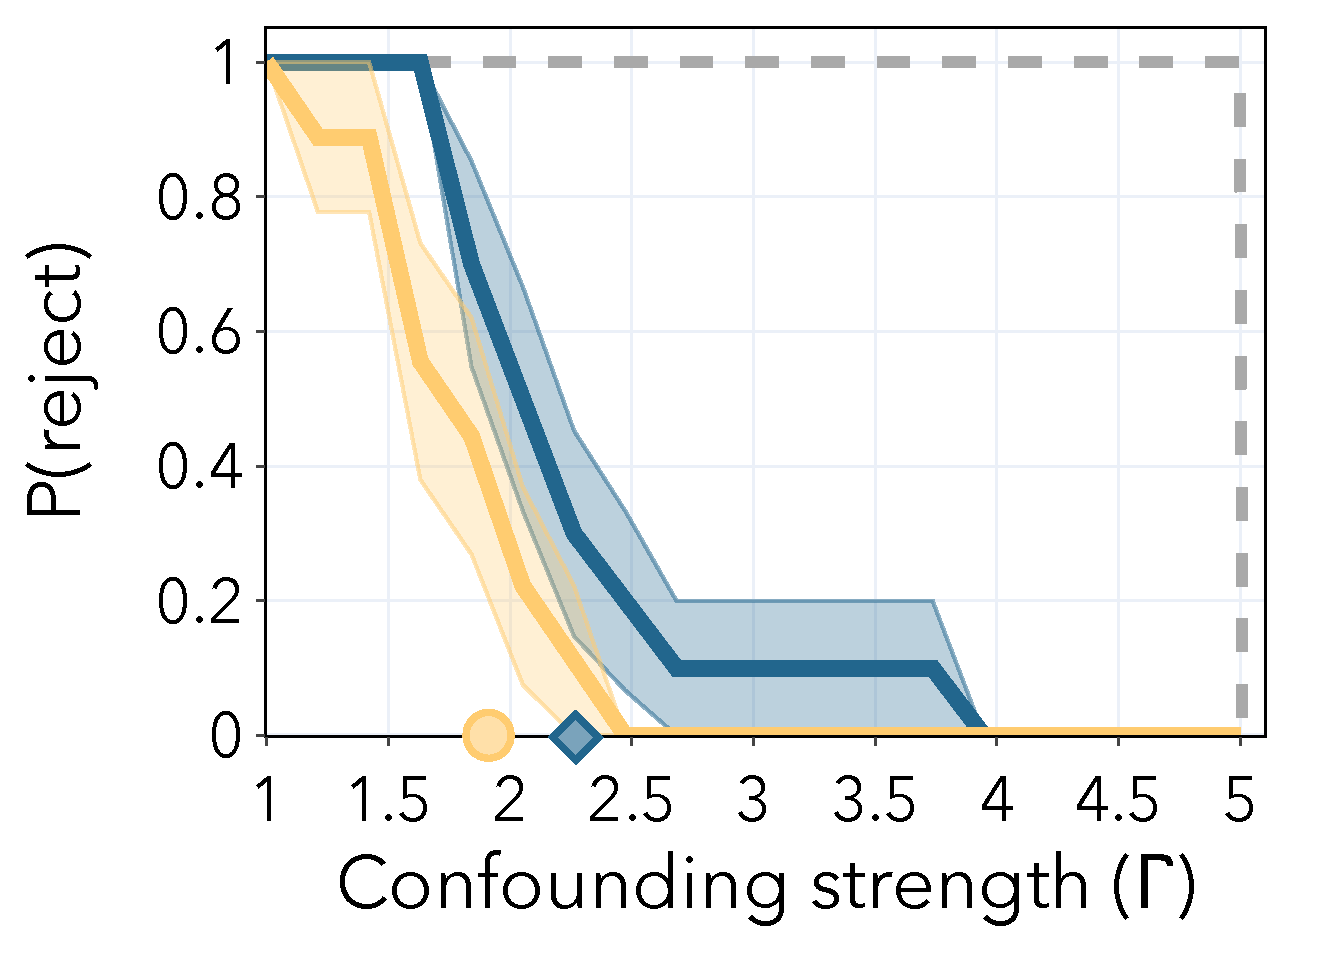
\includegraphics[width=\textwidth]{hillstrom_small}
        \caption{\footnotesize{Small sample (Hillstrom)} }
        \label{fig:hillstrom_small}
    \end{subfigure}
    \hfill
    \begin{subfigure}[b]{0.24\textwidth}
        \centering
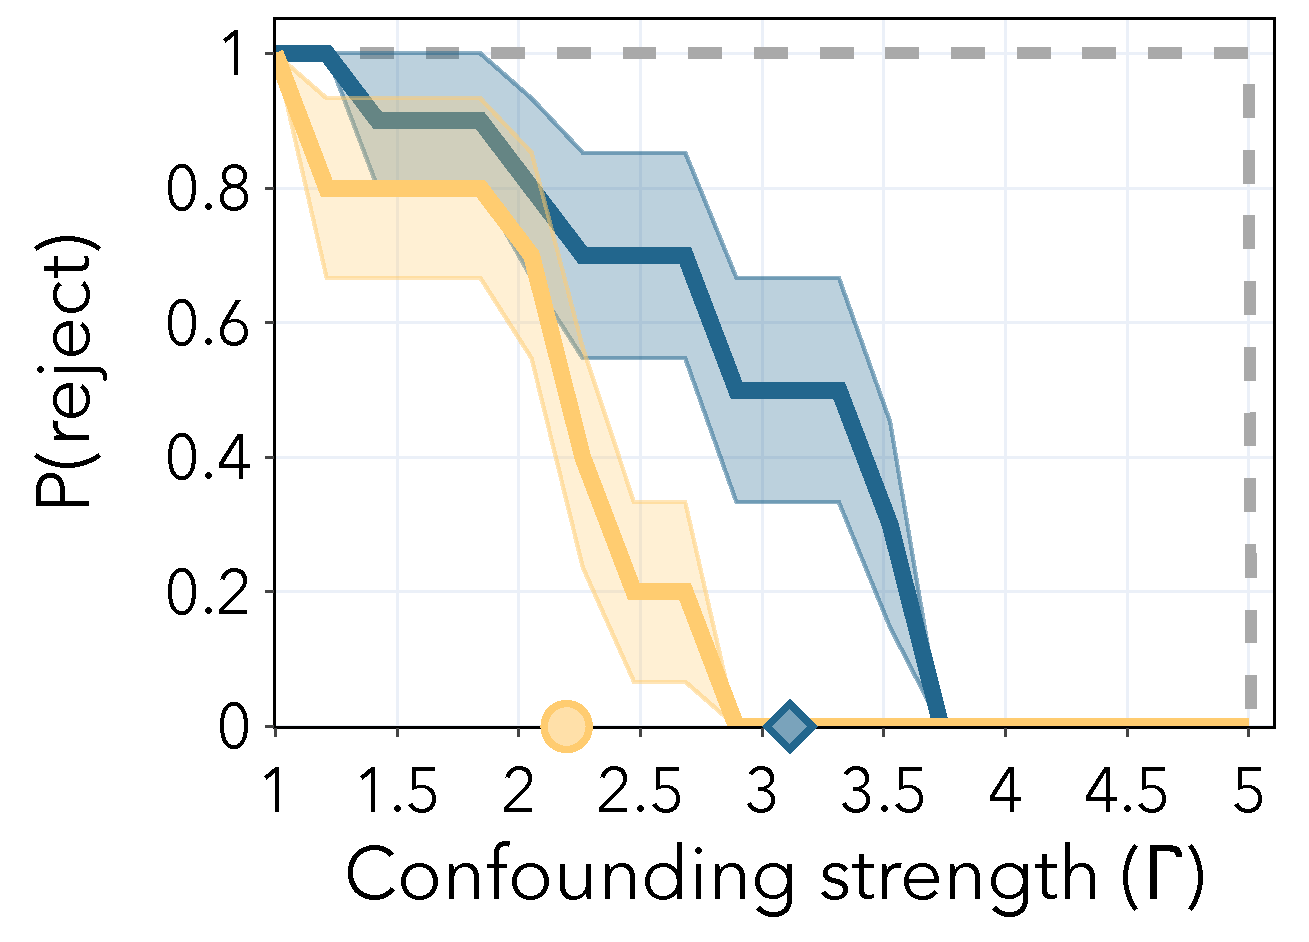
\includegraphics[width=\textwidth]{hillstrom_large}
        \caption{\footnotesize{Large sample (Hillstrom)} }
        \label{fig:hillstrom_large}
    \end{subfigure}
    \hfill
    \begin{subfigure}[b]{0.24\textwidth}
        \centering
   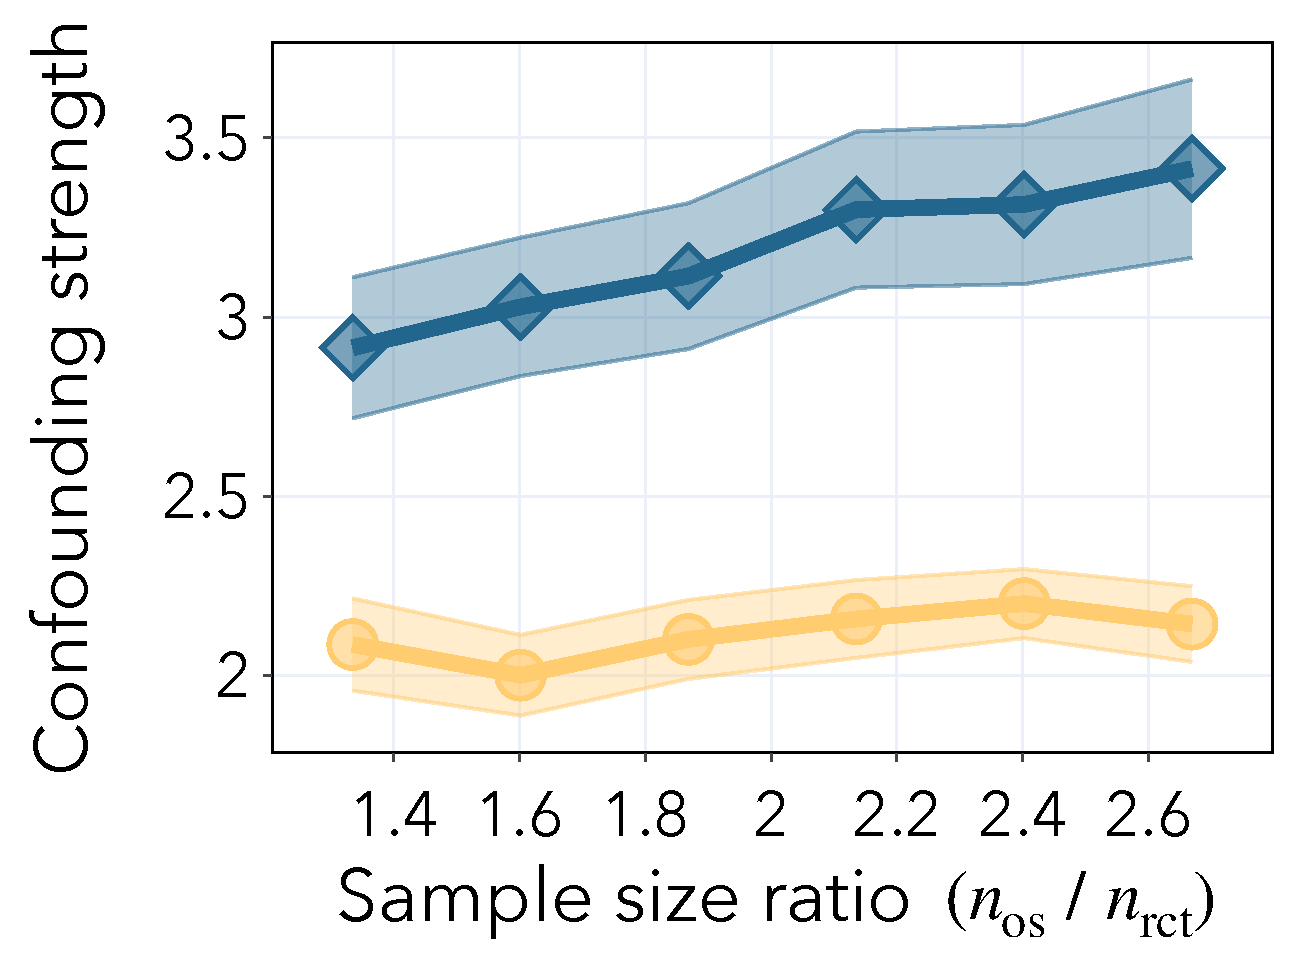
\includegraphics[width=\textwidth]{hillstrom_nobs}
        \caption{\footnotesize{Increasing $\nobs$} (Hillstrom)}
        \label{hillstrom:nobs}
    \end{subfigure}
    \hfill
    \begin{subfigure}[b]{0.245\textwidth}
        \centering
    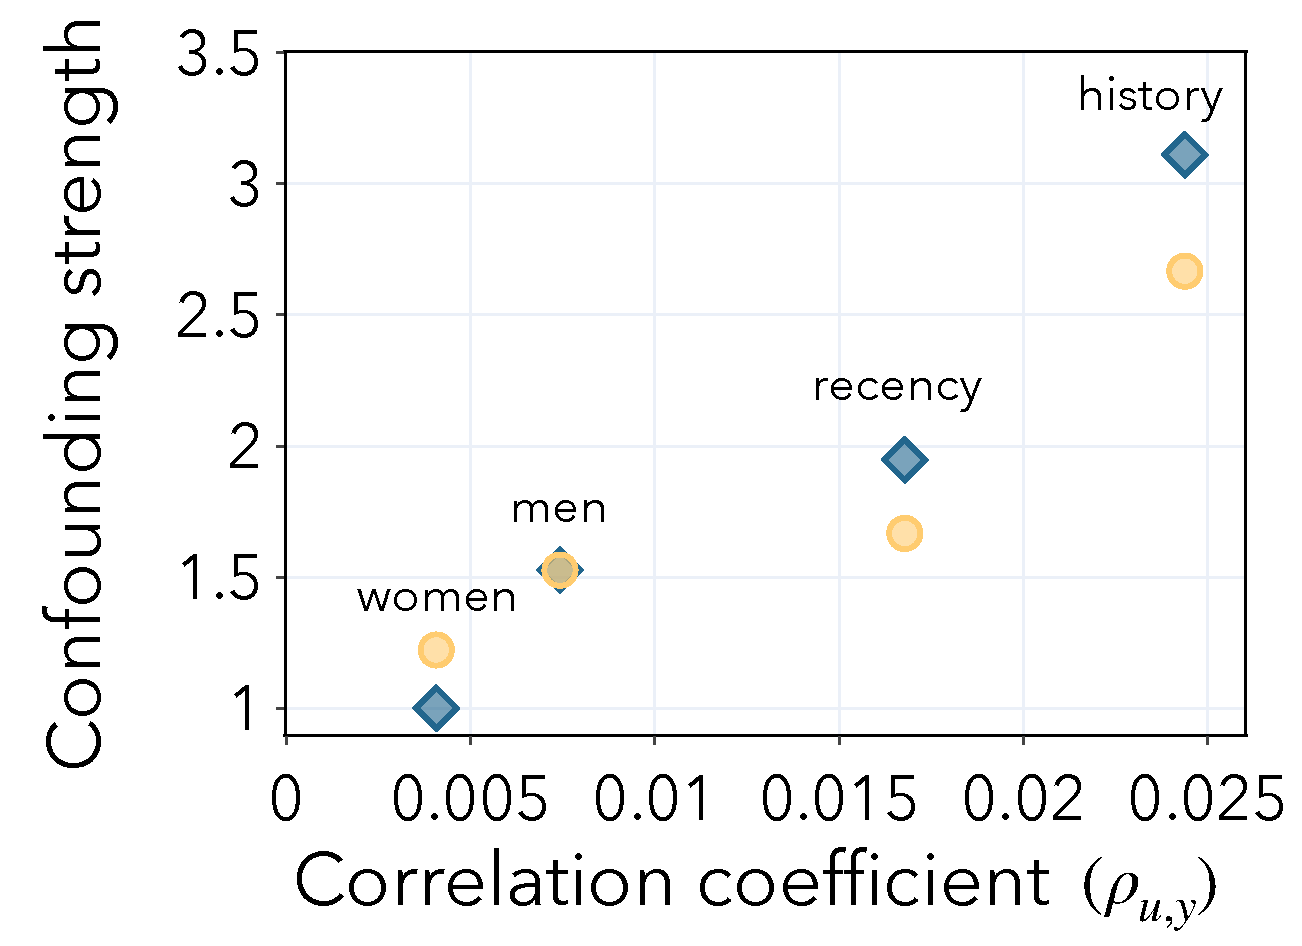
\includegraphics[width=\textwidth]{hillstrom_correlation}
        \caption{\footnotesize{$\rho_{u,y}$ effect (Hillstrom)}}
        \label{hillstrom:corr}

    \end{subfigure}
    
    \caption{\small{For all the plots: the significance level is $\alpha=0.05$, $\phi^\star$ denotes the oracle test which rejects for $\confvalue<
    \Gammatrue$, $\gammalb^{\rct}$ and $\gammalb^{\obsres}$ denote which test is used to compute $\gammalb$. First row with \emph{synthetic experiment} choosing  $\Gammatrue=5$: Probability of rejection for different $\confvalue$ and average $\gammalb$ for the test for (a) small sample size: $\nrct=2K,\nobs=2K$ and (b) large sample size: $\nrct=20K,\nobs=20K$. $\gammalb$ for (c) increasing sample size of the observational study with $\nrct=20K$ and (d) increasing correlation coefficient; $\nrct=20K,\nobs=20K$. Second row with the \emph{semi-synthetic} Hillstrom dataset choosing $\Gammatrue=5$ and using ``history" as unobserved confounder (except in (h)): Probability of rejection for different $\confvalue$ and average $\gammalb$ for (e) small sample size: $\nrct=2300$, $\nobs=6150$ and (f) large sample size: $\nrct=7680$, $\nobs=20500$. $\gammalb$ for (g) increasing $\nobs$ with $\nrct=7680$ and (h) increasing correlation coefficient.}
 }
    \label{fig:ate_synthetic}
\end{figure*}


\subsection{Experimental results}
 \label{sec:results}
 We now discuss our experimental results depicted in
~\Cref{fig:ate_synthetic}. The top row presents results for the synthetic experiments, and the bottom row for the semi-synthetic experiments. 



\paragraph{Effect of observational study sample size} 

First, we observe in Figures \ref{fig:synthetic_small_sample}-\ref{fig:synthetic_large_sample} and Figures \ref{fig:hillstrom_small}-\ref{fig:hillstrom_large} that our tests are valid in all settings, i.e. they do not reject for strengths larger than $\Gammatrue$. 
However, the statistical power substantially improves in the large sample size regime.  
 In general, the performance of both tests aligns.
In Figures \ref{fig:synthetic_obs_sample} and \ref{hillstrom:nobs}, the lower bounds $\gammalb^{\rct}$ and $\gammalb^{\obsres}$ vary
with the sample size of the observational study. We confirm that the $\test_{\obsres}$  derives greater benefits from a larger observational study sample size than $\hat{\phi}_{\mathrm{rct}}$, as discussed in~\Cref{sec:test_presentetion}. 

\paragraph{Effect of outcome-confounder correlation} 
Note that the tests in ~\Cref{fig:synthetic_small_sample}-\ref{fig:synthetic_large_sample} and ~\Cref{fig:hillstrom_small}-\ref{fig:hillstrom_large} are somewhat conservative: The probability of rejection for $\confvalue$ close to $\Gammatrue$ is small, which leads to a rather loose lower bound estimate $\gammalb$. This is due to a fundamental limitation of the marginal sensitivity model that cannot be overcome without additional assumptions on how U affects Y, as discussed in~\Cref{apx:limitations_msm}. We study here the effect of increasing the outcome-confounder correlation  (Equation~\ref{eq:correlation}).
Specifically, we generate observational datasets with a constant $\Gammatrue$ but varying $\rho_{u,y}$, and report $\gammalb$ for both tests. For the synthetic experiments in~\Cref{fig:synthetic_correlation}, we plot $\gammalb^{\rct}$ and $\gammalb^{\obsres}$ for $n=50$ distinct values of $\sigma^2_{Y(1)} \sim \operatorname{Unif}[0,1]$. For the semi-synthetic experiments in~\Cref{hillstrom:corr}, we depict $\gammalb^{\rct}$ and $\gammalb^{\obsres}$ for different hidden confounders $U$. Both plots confirm our hypothesis that higher $\rho_{u,y}$ correlates with a tighter lower bound $\gammalb$.




